\documentclass[10pt,twocolumn,letterpaper]{article}

\usepackage{cvpr}
\usepackage{times}
\usepackage{epsfig}
\usepackage{graphicx}
\usepackage{amsmath}
\usepackage{amssymb}

% Include other packages here, before hyperref.

% If you comment hyperref and then uncomment it, you should delete
% egpaper.aux before re-running latex.  (Or just hit 'q' on the first latex
% run, let it finish, and you should be clear).
\usepackage[breaklinks=true,bookmarks=false]{hyperref}

\cvprfinalcopy % *** Uncomment this line for the final submission

\def\cvprPaperID{****} % *** Enter the CVPR Paper ID here
\def\httilde{\mbox{\tt\raisebox{-.5ex}{\symbol{126}}}}

% Pages are numbered in submission mode, and unnumbered in camera-ready
%\ifcvprfinal\pagestyle{empty}\fi
\setcounter{page}{4321}
\begin{document}

%%%%%%%%% TITLE
\title{Pooling Pyramid Network for Object Detection}

\author{
Pengchong Jin
\hspace*{32pt}
Vivek Rathod
\hspace*{32pt}
Xiangxin Zhu
\\
Google AI Perception\\
{\tt\small \{pengchong, rathodv, xiangxin\}@google.com}
}


\maketitle
%\thispagestyle{empty}

%%%%%%%%% ABSTRACT
\begin{abstract}
We proposed 
   The ABSTRACT is to be in fully-justified italicized text, at the top
   of the left-hand column, below the author and affiliation
   information. Use the word ``Abstract'' as the title, in 12-point
   Times, boldface type, centered relative to the column, initially
   capitalized. The abstract is to be in 10-point, single-spaced type.
   Leave two blank lines after the Abstract, then begin the main text.
   Look at previous CVPR abstracts to get a feel for style and length.
\end{abstract}

%%%%%%%%% BODY TEXT
\section{Introduction}

\section{Related Work}

Multibox~\cite{erhan2014multibox}

SSD~\cite{liu2016ssd}

Faster-RCNN~\cite{ren2015frcnn}

YOLO~\cite{redmon2016yolo}

YOLO-v2~\cite{redmon2017yolov2}

FPN~\cite{lin2017fpn}

Survey~\cite{huang2017gmi}

RetinaNet~\cite{lin2017focal}

\section{Pooling Pyramid Network (PPN)}
Our proposed model, called \textit{Pooling Pyramid Network (PPN)},
is a single-stage convolutional object detector,
that is designed to be light-weighted, fast to run,
while maintains the good detection accuracy.
The network architecture is illustrated in Figure~\ref{fig:ppn}.
There are two major changes to the original SSD~\cite{liu2016ssd}:
(1) the convolutions between feature maps are replaced with the max pooling operations.
(2) the box predictor is shared across feature maps with different scales;
In the following sections, we will discuss the rationales behind them and effects of these changes.

\begin{figure}[t]
\begin{center}
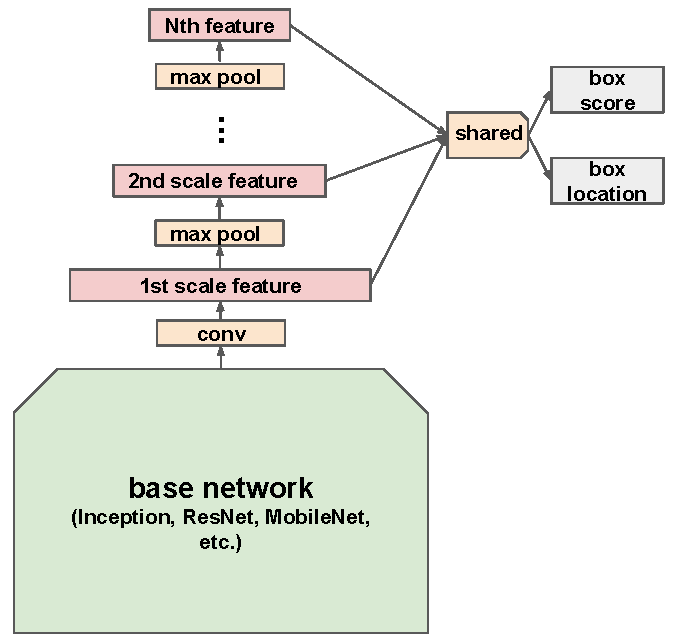
\includegraphics[width=0.8\linewidth]{figure/ppn.pdf}
\end{center}
\caption{
The Pooling Pyramid Network (PPN) architecture.
}
\label{fig:ppn}
\end{figure}

\subsection{Max Pooling Pyramid}

Our goal is to build a multi-scale feature pyramid structure, from which we can make the predictions using the shared box predictor.
We achieve this by shrinking down a base feature map from the backbone network serval times using a series of max pooling operations.
This is different from
SSD where feature maps are built by extracting layers from backbone network and shrinking them using additional convolutions,
and FPN where feature maps are built by a top-down pathway with skip connections.
We choose max pooling mainly for two reasons.
First, using the pooling operations ensures feature maps with different scales live in the same embedding space,
which makes training the shared box predictor more effective.
In addition, since max pooling does not require any additions and multiplicatons,
it is very fast to compute during the inference,
therefore, making it suitable for many latency sensitive applications.


\subsection{Shared Box Predictor}
The original SSD uses separate box predictors for feature maps of different scales.
While in this design
each box predictor is allocated to spend its full capacity on box prediction of one specific scale,
one potential problem is miscalibration of the prediction scores across different scales.
Because each box predictor is trained independently using only a portion of the groundtruth boxes that it is assigned to,
different box predictors could see very different amount of positive and negative examples during the training.
This implicit data imbalance problem could potentially cause the problem that
scores from different predictors fall in a very different ranges,
which makes them incomparable and difficult to use in the subsequent score-based postprocessing such as non maximum suppression.
We design PPN to use the shared box predictor accross feature maps of different scales.
As a result, the box predictor sees all the training data during the training
and implicitly argument the data when there are imbalance groundtruth boxes with different scales.
As a result, this reduces the effect of miscalibration and instable prediction scores.


\subsection{Overall Architecture}



The final network architecture of our Pooling Pyramid Network (PPN) detector is illustrated in Figure~\ref{fig:ppn}.
Followed by the backbone network, an optional 1x1 convolution is used to transform the features from the backbone network to a space with desired dimensions.
We then apply a series of stride-2 max pooling operations to shrink the feature map down to 1x1.
A shared box predictor is applied to feature maps of different scales
in order to produce classification scores and location offsets of box predictions.
We add one additional shared convolution in the box predictor after pooling operations
to prepare the feature to be used for predictions.


\section{Experiments}

\subsection{Comparing SSD and PPN}


\begin{table*}[t]
\begin{center}
\begin{tabular}{l|c|c|c|c|c}
Model & AP & AP50 & AP75 & FLOPs & number of parameters \\
\hline
\hline
MobileNet SSD & 1 & 1 & 1 & 1 & 1 \\
\hline
MobileNet PPN & 1 & 1 & 1 & 1 & 1 \\
\end{tabular}
\end{center}
\caption{COCO detection: MobileNet SSD vs MobileNet PPN}
\end{table*}




{\small
\bibliographystyle{ieee}
\bibliography{refs}
}

\end{document}
